%
% Beweis im allgemeinen Fall
%
\subsection{Beweis im allgemeinen Fall
\label{buch:intalg:liouville:subsection:allgemein}}
Der allgemeine Fall handelt von mehr als nur einer Erweiterung.
Gegeben ist wieder ein Funktionenkörper $F$ mit einer Derivation und
$f\in F$.
Der Konstantenkörper von $F$ wird wieder mit $K$ bezeichnet.
Um eine elementare Stammfunktion $g$ zu konstruieren, müssen mehrere
Funktionen $\vartheta_1,\dots,\vartheta_N$ hinzugefügt werden.
Dies geschieht mit einer Kette
\begin{equation}
\begin{tikzcd}[column sep=0pt]
f \arrow[d,tail] &
	& &
	& &
	& &
	& &
	& g \arrow[d,tail]
\\
F & \subset
	& F(\vartheta_1) \arrow[d,equal] & \subset
	& F(\vartheta_1,\vartheta_2) \arrow[d,equal] & \subset
	& \dots & \subset
	& F(\vartheta_1,\dots,\vartheta_{N-1}) \arrow[d,equal] & \subset
	& F(\vartheta_1,\dots,\vartheta_N) \arrow[d,equal]
\\
  &
	& F_1 & \subset 
	& F_2 & \subset 
	& \dots & \subset
	& F_{N-1} & \subset 
	& F_N
\end{tikzcd}
\label{buch:intalg:liouvill:allg:eqn:cd}
\end{equation}
von Körpererweiterungen.
Das Prinzip von Liouville besagt dann, dass $g$ allein in der Form
\begin{align*}
g
&=
v_0 + \sum_i c_i\log v_i
\intertext{mit Ableitung}
f
&=
Dv_0 + \sum_i c_i\frac{Dv_i}{v_i}
\end{align*}
mit $v_i\in F$ und $c_i\in K$.
Die Form von $g$ in $F_N$ ist also sehr speziell.

Die in
Abschnitt~\ref{buch:intalg:liouville:subsection:spezialfaelle}
bewiesenen Spezialfälle besagen, dass im Fall einer einzigen
Körpererweiterung $F\subset F_1$ eine Funktion $f$ mit Stammfunktion
$g\in F_1$ in der Form
\[
f = Dv_0 + c_1 \frac{Dv_1}{v_1}
\qquad\text{oder}\qquad
g = v_0 + c_1\log v_1
\]
geschrieben werden kann.

\begin{definition}[Liouville-Form]
Ist $g\in G$ eine Stammfunktion von $f\in F$, dann heisst
\[
g = v_0 + \sum_i c_i\log v_i \quad \text{mit } v_k \in F, c_i \in K
\]
eine \emph{Liouville-Form} von $g$ bezüglich $F\subset G$.
\end{definition}

Die Spezialfälle von
Abschnitt~\ref{buch:intalg:liouville:subsection:spezialfaelle}
besagen also, dass die Stammfunktion $g$ einer Funktion $f\in F$ nur
dann in $F(\vartheta)$ sein kann, wenn $g$ eine Liouville-Form
bezüglich $F\subset F(\vartheta)$ hat.
Wir können dies durch das Mengendiagramm
\begin{center}
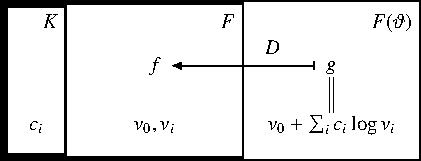
\includegraphics{chapters/070-intalg/images/lf0.pdf}
\end{center}
visualisieren.

Die Spezialfälle von 
Abschnitt~\ref{buch:intalg:liouville:subsection:spezialfaelle}
lassen sich auch auf die Erweiterung
$F_{N-1}\subset F_N = F_{N-1}(\vartheta_N)$ anwenden, die sich
als
\begin{center}
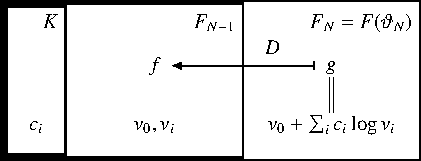
\includegraphics{chapters/070-intalg/images/lfN.pdf}
\end{center}
visualisieren lassen.

Was wir aber erreichen möchten, ist in Abbildung
%
% lf.tex
%
% (c) 2026 Prof Dr Andreas Müller
%
\begin{figure}
\centering
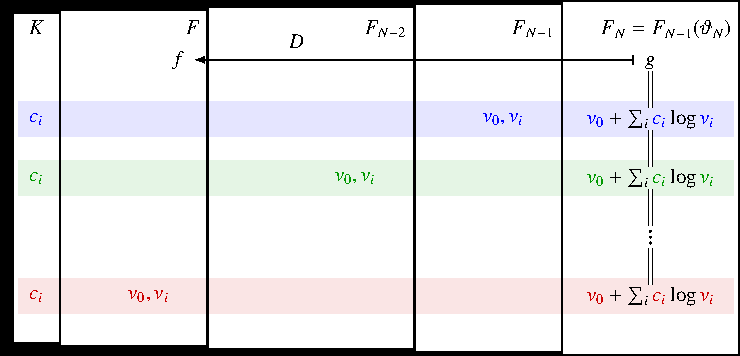
\includegraphics{chapters/070-intalg/images/lf.pdf}
\caption{Allgemeiner Fall des Prinzips von Liouville.
Die Stammfunktion $g\in F_N$ lässt sich in Liouville-Form
bezüglich $F_{N-1}\subset F_N$ mit den blauen Elementen
${\color{blue}c_i}\in K$ und
${\color{blue}v_0}, {\color{blue}v_i}\in F_{N-1}$
schreiben.
Sie muss schrittweise durch neue Elemente in anderen Farben 
in Liouville-Form bezüglich Erweiterungen $F_{k-1}\subset F_k$
umgeschrieben werden, bis die endgültige Liouville-Form mit
roten Elementen ${\color{darkred}c_i}\in K$ und
${\color{darkred}v_0}, {\color{darkred}v_i}\in F$ entsteht.
Dies beweist das Prinzip von Liouville.
\label{buch:intalg:liouville:fig:lf}}
\end{figure}
%
\ref{buch:intalg:liouville:fig:lf} dargestellt.
Zunächst gibt es blaue Elemente
${\color{blue}c_i}\in K$ und
${\color{blue}v_0},{\color{blue}v_i}\in F_{N-1}$, die eine
Liouville-Form für $g$ ergeben.
Diese muss jetzt zunächst in eine Liouville-Form mit den grünen
Elementen
${\color{darkgreen}c_i}\in K$ und
${\color{darkgreen}v_0},{\color{darkgreen}v_i}\in F_{N-2}$ 
bezüglich $F_{N-2}\subset F$ umgewandelt werden.
Durch Wiederholung dieses Prozesses kann man die roten Elemente
${\color{darkred}c_i}\in K$ und
${\color{darkred}v_0},{\color{darkred}v_i}\in F_{N-2}$ 
einer Liouville-Form von $g$ bezüglich $F\subset F_N$ bekommen,
was das Prinzip von Liouville beweist.
















